\chapter{Технологический раздел}

\section{Обоснование выбора системы управления базами\\ данных}

Систем управления базами данных очень много. Чтобы выбрать наиболее подходящую для данного приложения был проведен сравнительный анализ одних из наиболее популярных СУБД: MySQL, Oracle, PostgreSQL. 

При сравнении учитывалось:
\begin{enumerate}[label*=---]
	\item есть ли бесплатное и открытое программное обеспечение;
	\item поддерживаются ли процедурные расширения языка SQL;
	\item присутствует ли опыт работы с данной СУБД.
\end{enumerate}

\begin{table}[hbtp]
	\begin{center}
		\begin{flushleft}
			\captionsetup{justification=raggedright, singlelinecheck=false}
			\caption{\label{tab:bd}Сравнение СУБД}
		\end{flushleft}
		\begin{tabular}{|  p{0.20\textwidth} | p{0.23\textwidth} | p{0.25\textwidth}  |  p{0.18\textwidth}|} 
			\hline  Система управления базами данных & Бесплатное и открытое программное обеспечение & Поддержка процедурных расширений языка SQL  &  Наличие личного опыта работы \\ \hline
			MySQL~\cite{mysql} &  есть &  нет & нет \\ \hline
                Oracle~\cite{oracleReal} &   нет  &   есть & нет  \\ \hline
                PostgreSQL~\cite{postgres} &     есть & есть & есть \\ \hline
		\end{tabular}
	\end{center}
\end{table}

Исходя из сравнения в таблице~\ref{tab:bd} в качестве системы управления базами данных в данной работе будет использоваться PostgreSQL.

Как следует из таблицы~\ref{tab:bd} лучшим выбором СУБД для данного проекта будет PostgreSQL, так как он удовлетворяет всем критериям для выбора.


\section{Архитектура приложения}

Для проектирования винного интернет-магазина подходит клиент-серверная архитектура, так как там присутствует возможность более чёткого разграничения полномочий доступа к разным уровням информационной системы. Каждому клиенту — свой уровень доступа. 

Приложение винного магазина будет состоять из следующих компонентов:
\begin{enumerate}[label*=---]
	\item интерфейс;
	\item бизнес-логика;
	\item доступ к данным.
\end{enumerate} 
Верхнеуровневое разбиение на компоненты представлено на рисунке~\ref{img:upper}.
\begin{figure}[!h]
	\centering
	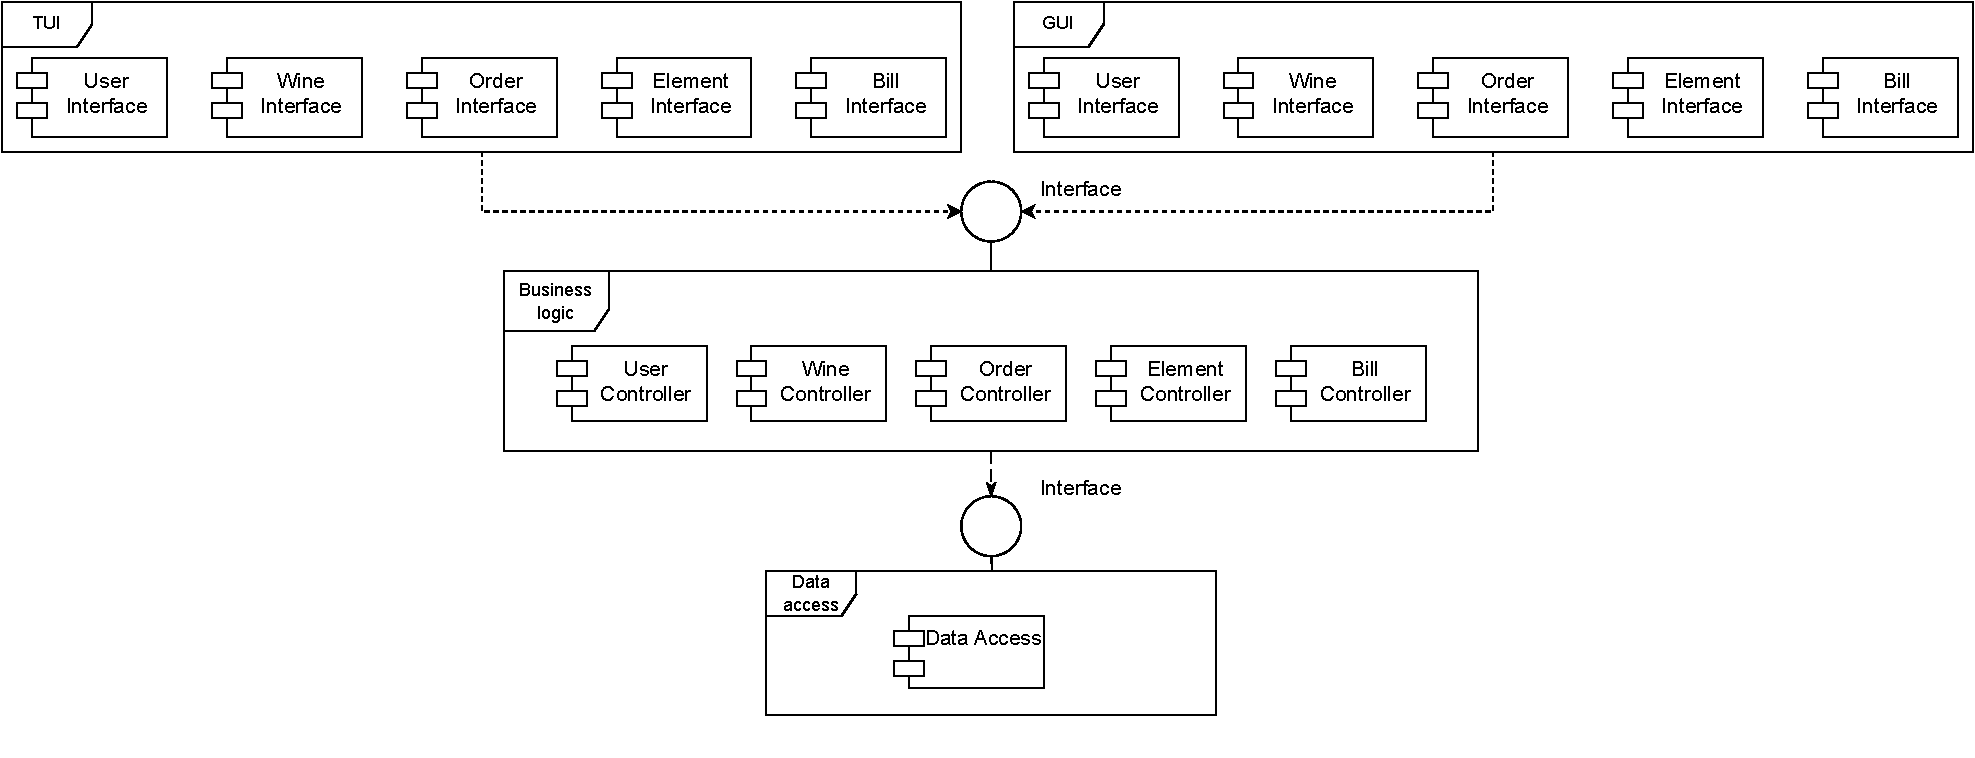
\includegraphics[scale=0.5]{inc/img/components.pdf}
	\caption{Верхнеуровневое разбиение на компоненты}
	\label{img:upper}
\end{figure}

\section{Средства реализации}
Через API~\cite{api} будет предоставлен доступ на сервер. Средством реализации API был выбран Swagger~\cite{swagger}, так как он автоматически описывает API на основе его кода. С помощью специального файла и OpenAPI
Generator генерируются интерфейсы клиента и сервера. Обработчики запросов используют сгенерированные интерфейсы для осуществления http запросов.

Были реализованы следующие запросы:
\begin{enumerate}[label=\arabic*)]
	\item /authorize

 Метод POST. Осуществляет авторизацию пользователя. В теле запроса находится структура состоящая из логина и пароля, которые являются строками. Ответом служит структура ошибочного ответа или структура пользователя, которая содержит поля:
 \begin{itemize}[label*=---]
	\item id --- строка;
	\item login --- строка;
	\item password --- строка;
        \item name --- строка;
        \item email --- строка;
        \item points --- строка;
        \item status --- строка;
\end{itemize}
 
	\item /register

Метод POST. Осуществляет регистрацию пользователя. В теле запроса находится структура, состоящая из:
\begin{itemize}[label*=---]
	\item login --- строка;
	\item password --- строка;
        \item name --- строка;
        \item email --- строка;
        \item status --- строка.
\end{itemize}
Ответом служит структура ошибочного ответа или структура, которая содержит булевое поле registered.
 
	\item /wines

Метод GET. Возвращает перечень вин. В теле запроса находится структура состоящая из строковых полей limit и skip.
Ответом служит структура ошибочного ответа или структура, которая содержит массив вин.

        \item /wines

Метод POST. Создает новое вино в каталоге. В теле запроса находится структура, состоящая из:
\begin{itemize}[label*=---]
	\item name --- строка;
	\item count --- строка;
        \item year --- целое число;
        \item strength --- целое число;
        \item price --- строка;
        \item type --- строка.
\end{itemize}
Ответом служит структура ошибочного ответа или структура с булевым полем added.

\item /wines

Метод PUT. Изменяет вино в каталоге. В теле запроса находится структура вина.
Ответом служит структура ошибочного ответа или структура с булевым полем updated.

\item /wines/{id}

Метод DELETE. Удаляет вино из каталога. Параметром является id. Ответом служит структура ошибочного ответа или структура с булевым полем deleted.


\item /wines/{id}

Метод GET. Получает конкретное вино из каталога. Параметром является id. Ответом служит структура ошибочного ответа или структура вина.


\item /elems

Метод POST. Создает элемент заказа с вином. В теле запроса находится структура элемента заказа. Ответом служит структура ошибочного ответа или структура с булевым полем created.

\item /elems

Метод GET. Получает все элементы данного заказа. В теле запроса находится структура со строчкой id заказа. Ответом служит структура ошибочного ответа или структура с массивом элементов заказа.

\item /elems/{id}/decrease

Метод PUT. Уменьшает количество вина в заказе на 1. Параметром является id элемента заказа. Ответом служит структура ошибочного ответа или структура с булевым полем decreased.

\item /elems/{id}/add

Метод PUT. Увеличивает количество вина в заказе на 1. Параметром является id элемента заказа. Ответом служит структура ошибочного ответа или структура с булевым полем added.

\item /elems/{id}

Метод DELETE. Удаляет элемент заказа. Параметром является id элемента заказа. Ответом служит структура ошибочного ответа или структура с булевым полем deleted.

\item /orders/{id}

Метод GET. Получает заказ по id. Параметром является id заказа. Ответом служит структура ошибочного ответа или структура заказа.

\item /orders

Метод PUT. Оформляет заказ. В теле запроса находится структура заказа. Ответом служит структура ошибочного ответа или структура с булевым полем placed.

\item  /bills/{id}

Метод PUT. Подтверждает оплату счета. Параметром является id счета. Ответом служит структура ошибочного ответа или структура с булевым полем payed.

\item /users

Метод PUT. Обновляет баллы у пользователя. В теле запроса находится структура, которая содержит id пользователя и количество баллов, на которое нужно изменить баллы клиента. Ответом служит структура ошибочного ответа или структура с булевым полем updated.


\item /favourite/{id}

Метод GET. Получает любимые вина пользователя. Параметром является id пользователя. Ответом служит структура ошибочного ответа или структура с массивом любимых вин, которые состоят из идентификаторов пользователя и вина.

\item /favourite
Метод POST. Добавляет вино в <<любимое>>. В теле запроса находится структура, состоящая из идентификаторов пользователя и вина.
Ответом служит структура ошибочного ответа или структура с булевым полем added.

\item /favourite
Метод DELETE. Удаляет вино из <<любимого>>. В теле запроса находится структура, состоящая из идентификаторов пользователя и вина.
Ответом служит структура ошибочного ответа или структура с булевым полем deleted.

\end{enumerate}


Приложение реализовано на языке Go\cite{go}, так как у него присутствуют библиотеки для написания тестов, для http-запросов\cite{http}, для подключения к базе данных\cite{gorm}.  Для доступа к базе данных был использован паттерн <<репозиторий>>. Интерфейс приложения --- консольный, который реализует MVC паттерн.

\section{Детали реализации}
 \subsection{Создание таблиц}

В листингах~\ref{lst:user.sql} ---  \ref{lst:userwines.sql}представлен код создания 6 таблиц для приложения винного магазина. При создании сразу устанавливаются ограничения целостности. Таблицы создаются при миграции с помощью утилиты goose\cite{goose}. 


\includelisting
{user.sql} % Имя файла с расширением (файл должен быть расположен в директории inc/lst/)
{Создание таблицы пользователей} % Подпись листинга

\includelisting
{wine.sql} % Имя файла с расширением (файл должен быть расположен в директории inc/lst/)
    {Создание таблицы вин} % Подпись листинга
    
\includelisting
{order.sql} % Имя файла с расширением (файл должен быть расположен в директории inc/lst/)
    {Создание таблицы заказов} % Подпись листинга
    
\includelisting
{elem.sql} % Имя файла с расширением (файл должен быть расположен в директории inc/lst/)
    {Создание таблицы элементов заказа} % Подпись листинга

    
\includelisting
{bill.sql} % Имя файла с расширением (файл должен быть расположен в директории inc/lst/)
    {Создание таблицы счетов} % Подпись листинга
    
\includelisting
{userwines.sql} % Имя файла с расширением (файл должен быть расположен в директории inc/lst/)
    {Создание таблиы любимых вин} % Подпись листинга
    
\subsection{Создание ролей на уровне базы данных}

В данной работе представлено 3 роли на уровне базы данных: гость, пользователь и администратор. Создание ролей и выделение им прав, в соответствии с ролевой моделью, представлены в листинге~\ref{lst:role.sql}. 

\includelisting
{role.sql} % Имя файла с расширением (файл должен быть расположен в директории inc/lst/)
    {Создание ролей на уровне базы данных} % Подпись листинга

Гостю предоставляется меню из следующих пунктов:
\begin{itemize}[label*=---]
	\item Выход;
	\item Регистрация;
        \item Авторизация;
        \item Получить каталог вин.
\end{itemize}

Зарегистрированный пользователь получает меню, представленное ниже:
\begin{itemize}[label*=---]
	\item Выход;
	\item Добавить вино в заказ;
        \item Увеличить количество вина в заказе;
        \item Уменьшить количество вина в заказе;
        \item Удалить вино из заказа;
        \item Получить каталог вин;
        \item Получить текущий заказ;
        \item Оформить заказ;
        \item Добавить вино в любимое;
        \item Получить список любимых вин;
        \item Удалить вино из любимого.
\end{itemize}

Для администратора выводится следующее меню:
\begin{itemize}[label*=---]
	\item Выход;
        \item Регистрация;
        \item Получить каталог вин;
        \item Подтвердить оплату счета;
        \item Добавить вино;
        \item Удалить вино;
        \item Изменить вино.
\end{itemize}


 \subsection{Создание триггера}

 Разработан триггер для проверки элемента заказа перед его вставкой в таблицу. Необходимо удостовериться, что данного вина уже нет в заказе и что на складе хватает товара для продажи. Код триггера и соответствующей функции представлен в листинге~\ref{lst:tr.sql}. 

 \includelisting
{tr.sql} % Имя файла с расширением (файл должен быть расположен в директории inc/lst/)
{Триггер, срабатывающий при добавлении нового элемента заказа} % Подпись листинга

 \section{Тестирование}

 Тестирование было проведено с помощью модульных и интеграционных тестов. Для модульных тестов были сгенерированы заглушки на репозитории для досткупа к данным с помощью пакета minimock\cite{minimock}. Модульные тесты написаны для компонента бизнес логики, а именно для контроллеров вина, пользователя, заказа, элемента заказа и счета.
 Каждый интеграционный тест выполняется в отдельном Docker\cite{docker} контейнере, до теста запускается миграция для создания таблиц и скрипт по заполнению тестовыми данными. Интеграционными тестами проверено получение заказа и обновление баллов у пользователя. Все тесты пройдены успешно.
 

\section*{Вывод}
 В данном разделе была описана архитектура приложения, средства и детали его реализации. 